\chapter{Implementation}

This chapter deals with the description of implementing and modifying the LCS.

For this thesis there was created a test project in the Infomedia TFS where I could do my work. This was so that I would not mess up Infomedia's inflow while trying to make the algorithms work correctly.

\section{Basic LCS Implementation}
First off the Cosine algorithm was implemented in said test project. There was no changes to that implementation,  it was implemented to work as it currently does in our inflow. Doing this, would make testing the LCS implementation show what results would be returned once this was in production. After that the basic implementation of LCS was implemented.

Then the basic LCS algorithm was implemented in the project, to be used for further development. It is taken without modifications from the wikibooks site ~\cite{WikiLCS}.

\lstset{style=sharpc}
\begin{lstlisting}[caption=Basic LCS implementation in C$^\sharp$, captionpos=b]

public int LongestCommonSubstring(string str1,
	 string str2)
{
    if (String.IsNullOrEmpty(str1) 
    	|| String.IsNullOrEmpty(str2))
    return 0;
	
	int[,] num = new int[str1.Length, str2.Length];
	int maxlen = 0;

    for (int i = 0; i < str1.Length; i++)
  	{
    	for (int j = 0; j < str2.Length; j++)
        {
        	if (str1[i] != str2[j])
            	num[i, j] = 0;
            else
            {
            	if ((i == 0) || (j == 0))
                	num[i, j] = 1;
                else
                    num[i, j] = 1 + num[i - 1, j - 1];

                    if (num[i, j] > maxlen)
                    {
                    	maxlen = num[i, j];
                  	}
           	}
     	}
	}
    return maxlen;
}

\end{lstlisting}

The LCS method works by taking in two strings as arguments and then comparing them character by character (see figure ~\ref{LcsExplained}. First off the algorithm checks to see if either of the string arguments are either \textit{null} or \textit{Empty}, which basically means that it makes a check for if either argument either was not set when calling the method or that either string was without any content. Because if this is the case, then the returning value will be 0, and there is no need to do any further work. The method then creates two arrays, one for each of the strings. It then tries to match the first character of the first array with all characters of the second array, marking any matches with a number. The number is given by checking the value in the double array on step back diagonally (see figure ~\ref{LcsExplained}), if it is the first time a match was found, that number will be stored as the length of the longest common substring. When ever another match is found, the algorithm then checks to see if the length (number in the [i, j] space of the array) are bigger than the length of the current longest common substring. If this is the case, the newly found max length is then stored. After having checked all places in the [i, j] array, the algorithm then returns the length of the longest common substring.

This implementation can easily be modified to return the content of the longest common substring (all the chars in that String)\footnote{\url{http://en.wikibooks.org/wiki/Algorithm_Implementation/Strings/Longest_common_substring\#Retrieve_the_Longest_Substring}}.

This works really well for finding substrings that can have been obfuscated in long lines of text. How ever in this thesis, the main objective is to find substrings of plain words rather than finding bits and pieces.

When comparing two articles with the LCS, the algorithm finds a lot of substrings, but only keeps the longest by default

The next step was to modify the LCS algorithm to make it suit the needs of this thesis. When looking at article duplicates, it makes more sense to look for entire words rather than single characters. This is because when an article is duplicated, any obfuscation or alteration would be done by cutting out sections of the article or moving sections around or adding new sections.

\section{Modification of LCS - String Comparison}
As hinted both in the text of the last section and also in figure ~\ref{LcsEx}, the next step was to modify LCS to compare whole words (string) instead of single letters (char). There are of course pros and cons to this approach. One of the pros would be that we could improve the performance of the algorithm. If we assume that the average word length is roughly five characters long\footnote{\url{http://www.wolframalpha.com/input/?i=average+english+word+length} - although it is for English words, it is most likely not that different from Danish.}, that means that comparing articles on a character by character basis increases the number of comparisons by a factor of 25 as compared to doing it word by word. This will therefore mean we can get a rather big performance boost, and when talking about an inflow that just for my test corpus contains ~22800 articles, but can be as many as 40000 articles daily, this factor will make quite the impact. Another pro is that we are looking for word duplication, not for sentences obfuscated within other sentences, therefore we do not really need to look at single characters.

On the cons side is the fact that if we are looking for words rather than single characters the algorithm becomes more prone to spelling errors. If the word \textit{'doomsday device'} was included in an article and in an article that is a duplicate of that article was a spelling error \textit{'doomday device'}, this would cause the character based substring to be slightly longer than than the words based substring. The character based substring would return \textit{'sday device'} whereas the word based substring would only contain \textit{'device'}. This can be an issue within texts that have \underline{many} spelling error, but that case is highly unlikely to appear in the articles this thesis is dealing with, as one would assume that journalists are pretty okay with correct spelling (and also has spelling checking on their text programs). 

So even though modifying LCS to compare words with words rather than characters, can return incorrect results, the likely hood of this being a substantial error source is negligible.

\subsection{Issue With Word (String) Comparisons}
The issue with comparing words rather than single characters in data science, is that the way comparison is done with data types, which is not as easy as when a human would do text comparison. For a human, reading and comparing two list of single letters, would be substantially slower than comparing two lists of words. This is based on how we recognize both single letters and words. A computer does things in a completely different way.\\* The basic implementation of LCS compares chars with chars, a char being a primitive data type in most modern objective oriented programming languages (Java, \verb!C!$^\sharp$, Objective \verb!C!, \verb!C++! and so on). Comparing primitives is a simple operation, just checking their values. The modification being implemented here would compare Strings with Strings, a String being of data type \textit{'object'} in object oriented languages. A String is internally a list of chars, that makes up the whole String, so comparing a String object with another String object is basically doing a char comparison (with some minor differences, such as String comparison also checks the length of the Strings).

However, in a future implementation of the modified version of LCS, one could transform the Strings into an int (one could use the word map generated by the Cosine algorithm for this), so that each word gets it's own int value, comparing the words as int values would be much faster than both the String and char comparison. This is because an int is a primitive, like the char, and instead of having to check a lot of chars for each "word", there would only be a need to check a single int value for each word. This would improve the overall performance of LCS dramatically (approximately by a factor 25, by applying the same theory as above, each word on average being five characters long) as the list of words (int) would be substantially shorter than the lists of chars. 
The conversion of String to int could be done in the text preparation phase (see Section~\ref{TextPrep}).

Due to the fact that I did not contemplate this until late in the work process, there have been no time to implement a String to int conversion in the LCS modification.

For testing purposes it is nicer and easier to read text split up into words rather than text split in chars, so that is a feature of the String comparison modification of LCS.

So even though it adds no immediate performance boost, this is both a step on the way and helping hand in terms of evaluating the results from LCS.

\section{Collection of Substrings}
Another modification to the LCS that would help finding article duplicates would be to make LCS create a collection of substrings. The benefits of this would to some extend help eliminate the error prone ways of LCS. If looking at two articles that would be considered a perfect match (same length, same article text), except for the word in middle of the text in one of the articles. If this have been changed, misspelled or forgotten, this would cause the basic implementation of LCS to return that the length of the longest common substring would be just under 50\% of the article's length. How ever, if we create a collection of substring we can in part work around this issue. Then we would find two substrings, one before the middle word (that is missing or in other way not present in the same form as in the other article) and one after the middle word. Our combination of substrings would then return a length that is close to 100\% of the article length (all words minus the missing word).

When doing this modification one should consider using a threshold that indicates the minimum length a substring should have in order to be included. There will inevitably be a lot of short matches (single words, white spaces, two words that are often in same context and so on) when comparing articles with the LCS. So an effective threshold would be one that filters away the noise, but it not so high that important (in terms of finding duplicates) sentences are filtered out. For this thesis the threshold have been set to four, meaning that all substrings consisting of four or more words are being stored as a result.

When creating the collection of substrings their lengths will be added and compared to the total length, thus creating a hopefully more correct image of whether two articles match or not.

\lstset{style=sharpc}
\begin{lstlisting}[caption=Modified version of LCS, captionpos=b]

public Dictionary<String, String>
 LongestCommonSubstring(List<String> str1,
  List<String> str2, int threshold)
    {
	  if (str1.Count == 0 || str2.Count == 0)
	      throw new Exception
	      ("One or both documents was empty.");

      int[,] num = new int[str1.Count, str2.Count];

      var combined = new Dictionary<string, string>();

      for (int i = 0; i < str1.Count; i++)
      {
         for (int j = 0; j < str2.Count; j++)
         {
            if (str1[i] != str2[j])
                num[i, j] = 0;
            else
            {
              if ((i == 0) || (j == 0))
                  num[i, j] = 1;
              else
                  num[i, j] = 1 + num[i - 1, j - 1];

              if (num[i, j] >= threshold)
              {
                // Find the start index 
                // of the current substring
                String index = 
                ((i - num[i, j]) + 
                ", " + (j - num[i, j]));

                String insert = "";
                // Do we already have this key stored?
                if (!combined.ContainsKey(index))
                {
                    var words = new List<String>();
                    for (int x = 3; x > 0; x--)
                    {
                       words.Add(str1[i - x]);
                    }
                    foreach (String word in words)
                       insert += word + " ";
                    insert += str1[i] + " ";
                    combined.Add(index, insert);
                }
                else
                {
                    String valueStore = combined[index];
                    valueStore += str1[i] + " ";
                    combined[index] = valueStore;
                }
              }
            }
          }
        }
       return combined;
   }

\end{lstlisting}

We can see from listing above, that the LCS works largely in the same way as before. How ever there are (naturally) some changes. The first being we no longer just check to see if the current substring is longer than the current longest common substring. As part of the method arguments we now provide the algorithm with a threshold, this threshold is what we are now evaluating our substrings against. When ever a match is found between two words we then mark the match in the double array as done in the basic LCS implementation. The value of the marked space will then be evaluated against the threshold. If the value is greater than or equal to the threshold value, we want to to store that substring. This is done using a dictionary. The key of the dictionary is the combination of values of \textit{i} and \textit{j} combined with a \textit{','}. The key has to be a unique value, which is the reason for adding the comma. This also have the added bonus of making it easier to read for humans, when trying to read the results from the algorithm.\\* 
First off the algorithm checks if the [i, j] value (the key in the dictionary) is already in the dictionary, if so, it adds the String content to the value part of the key. If not, it then adds the key and adds the value of the [i, j] space we are looking at and the value of the three previous (diagonally back) values. For each value we add a white space. Again this makes it easier to read, but also, the longest common substring found in the basic LCS implementation would count white spaces as well. The way that the modified LCS is called by the program, it is given two lists of Strings, with only the actual words of the articles, the white spaces are removed. The algorithm then adds white spaces after each word to have a result that matches the basic LCS better. 

Once all the words have been matched, the algorithm then returns \textit{result} which then contains all substrings found with a length greater or equal to the given threshold.



\section{Post Processing}
Once all articles in the test corpus (or the selected articles) have been processed through the algorithms and scored, the results and the articles was stored in a data type (see figure ~\ref{Datatypes}), \textit{AdvancedComparisonResult}, and then that was stored in a list of the same type. This list would then be processed through other methods for creating visual representations of the results.

\begin{figure}[h]
	\centering
	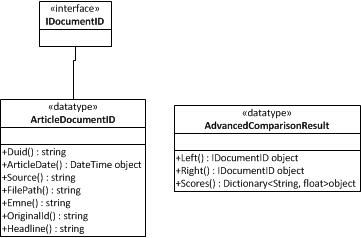
\includegraphics[scale=0.7]{figures/Datatypes}
	\caption{The data types used to store article information and information about article comparisons.}
	\label{Datatypes}
\end{figure}


\begin{figure}
	\centering
	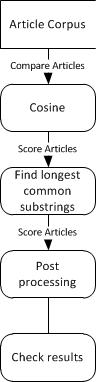
\includegraphics[scale=1.0]{figures/Dataflow}
	\caption{Flow chart for the implemented system.}
	\label{Dataflow}
\end{figure}




